\section{Evolutionary-Optimal Observation Matrix Design}  \label{sec:SNIPEREvlObsMtxDsg}
Evolutionary algorithms are the sub-category of heuristic optimization methods \cite{Talib:2009} for solving NP-hard optimization problems where the main objective function may not be formulated as a well-defined mathematical function. As Figure \ref{fig:EvolutionaryAlgsFC} shows, evolutionary algorithms consists of three main processes. The first process is the initialization process where the initial population of individuals is randomly generated according to some solution representation. Each individual represents a solution. In the second process, each solution in the population is then evaluated for a fitness value. The fitness values can be used to calculate the average population for the purpose of selection. The third process is the generation of a new population by the perturbation of solutions in the existing population. The algorithm is run until the stopping criterion is met. In this paper, we use two EOAs including Genetic Algorithm (GA) and Particle Swarm Optimization (PSO) which have been applied to many optimization and machine learning problems \cite{Talib:2009}\cite{Kachitvichyanuku:2012}.
%\begin{figure}[t]
  %\begin{center}
    %{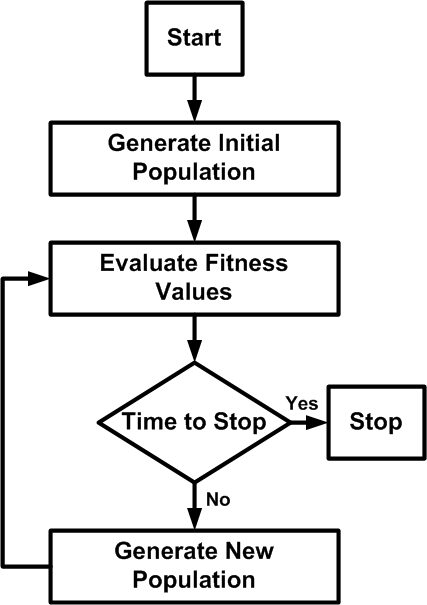
\includegraphics[keepaspectratio, width=0.2\textwidth]{EvolutionaryAlgsFC.png}}
  %\end{center}
  %\caption{\small{The general flowchart of evolutionary optimization algorithms.}}
  %\label{fig:EvolutionaryAlgsFC}
%\end{figure}

The main idea of GA is to mimic the natural selection mechanism and the survival of the fittest. In GA, the solutions are represented as chromosomes. The chromosomes are evaluated for fitness values and they are ranked from the best to the worst based on fitness value. The process to produce new solutions in GA is accomplished through three genetic operators as selection, crossover, and mutation. First, the better chromosomes are selected as parents to generate new offspring (new chromosomes). To simulate the survivor of the fittest, the chromosomes with better fitness are selected with higher probabilities. Once the parent chromosomes are selected, the crossover operator combines the chromosomes of the parents to produce new offspring (perturbation of old solutions). To avoid stagnation in the process of evolution, the mutation operator is performed on the chromosomes to increase the diversity of the population. To successfully apply the GA, the solution representation (i.e. chromosome model) must be designed carefully. Also, the parent selection process, and the probability of crossover and mutation are important parameters that must be precisely chosen \cite{Kachitvichyanuku:2012}.

In PSO, a solution is represented as a particle, and the population of solutions is called a swarm of particles. The first process in PSO is the initialization process where the initial swarm of particles is generated. Each particle is initialized with a random position and velocity. Each particle is then evaluated for fitness value. Each time a fitness value is calculated, it is compared against the previous best fitness value of the particle and the previous best fitness value of the whole swarm, and, accordingly, the personal best and global best positions are updated, appropriately. If a stopping criterion is not met, the velocity and position are updated to create a new swarm. The positions and velocities of particles are updated based on the personal best and global best positions, as well as the
old velocities. It should be noted that PSO algorithm does not require sorting of fitness values of solutions in any process. This might be a significant computational advantage over GA, especially when the population size is large \cite{Kachitvichyanuku:2012} \cite{Eberhart:2001}.
% The velocity is updated based on three components: the old velocity (inertia or momentum term), experience of an individual particle (cognitive or self learning term), and experience of the whole swarm (group or social learning term). Each term has a weight constant associated with it.
% Throughout this paper, the fitness of the solutions in our evolutionary algorithms are evaluated using the two metrics defined in Eq.(\ref{NormMetrics}) (see Section \ref{sec:SNIPERPerfEvalApp}), namely, Normalized Mean Absolute Error (NMAE) and Normalized Mean Square Error (NMSE) where $x_{ij}$ denotes the $ij^{th}$ entry of the matrix $X$ (which is known in the learning stage indicated by $T_{0}$) and $\hat{x}_{ij}$ denotes the $ij^{th}$ entry of the matrix $\hat{X}$ which is output of the MC process. 
%\begin{equation} \label{NormMetrics}
%\footnotesize{
%\begin{aligned}
%NMAE = \frac{\sum_{ij \in \bar{\Omega}} \left|x_{ij} - \hat{x}_{ij}\right|}{\sum_{ij \in \bar{\Omega}} \left|x_{ij}\right|} \\
%NMSE = \frac{\sqrt{\sum_{ij \in \bar{\Omega}} \left(x_{ij} - \hat{x}_{ij}\right)^{2} }}{\sqrt{\sum_{ij \in \bar{\Omega}} \left(x_{ij}\right)^{2}}}
%\end{aligned}
%}
%\end{equation}
Here, a solution in the GA is represented as a chromosome which is defined as a binary sampling matrix $C$ with size $n \times T_{0}$ and where $0$ and $1$ respectively represent unobserved and directly measured entries. The number of measurements paths (i.e. samples) for each chromosome is denoted by $K$ (i.e. the number of one's in each chromosome, see Section. \ref{sec:SNIPERPerfEvalApp}). To successfully apply the MC technique, the sampling matrix $C$ is constrained to have at least one $1$ in each row and column. The GA is started by generating $N_{p}$ chromosomes/solutions in the initialization step and estimating all unknown IAI in the set $\bar{\Omega}$ using MC algorithm. Then, the fitness of each chromosome is evaluated using the cost function Eq.(\ref{NormMetrics}). Accordingly, the best chromosomes, with lowest fitness values, are selected and the crossover operation, with probability $p_{c}$, is applied on each pair of parents to generate new children (offsprings). Eq.(\ref{GACrossOver}) defines the crossover operation where $r_{c}$ denotes a randomly chosen row from set $\{1,...,n\}$. These Offsprings form part of the new chromosomes of the next generation. To increase the diversity of the population, the mutation operation is performed on each child where the mutation operator changes an entry of sampling matrix $C$ from zero-to-one or vice-versa with probability $p_{m}$. The GA process is continued over $N_{i}$ iterations and the best chromosome in each iteration remains unchanged. In most cases throughout this paper, the GA parameters are set as: $N_{i}=60$, $N_{p}$=1500, $p_{c}=0.3$, and $p_{m}=0.01$.
% Among these, the best chromosome remains unchanged; and also, some simple manipulations are applied at each step to keep the number of measurement paths constant for each sampling rate in such a way that chromosomes remain symmetric (if it is required, for example, in the case of delay measurement) with having at least an one in each row/column of $C$ (please refer to \cite{SNIPERTechReport:2014} for further details). The GA process is continued over $N_{i}$ iterations.
\begin{equation} \label{GACrossOver}
% \small{
\begin{aligned}
\text{OffSpring}_{1} = C_{1}(1:r_{c},:) + C_{2}(r_{c}+1:n,:) \\
\text{OffSpring}_{2} = C_{2}(1:r_{c},:) + C_{1}(r_{c}+1:n,:) 
\end{aligned}
% }
\end{equation}

Likewise, the PSO is started by generating $N_{p}$ particles and estimating all unknown IAI in the set $\bar{\Omega}$ using the MC algorithm. The $i^{th}$ particle is identified by its position $P^{k}_{i}$ and its velocity $V^{k}_{i}$ at iteration $k$. Here, $P^{k}_{i}$ is an $n \times T_{0}$ binary matrix, representing the measurement matrix, and $V^{k}_{i}$ is also an $n \times T_{0}$ matrix. In the initialization stage all position and velocity matrices are zero matrices. The best position of $i^{th}$ particle obtained until iteration $k$ is denoted by $BP_{i}^{k}$ and the best position among all particles in the swarm until iteration $k$ is called global best position and it is denoted by $GP^{k}$. The best particles here is determined by evaluating the fitness of each particle and choosing the one with the minimum error value (as defined in Eq.(\ref{NormMetrics})) among all iterations (for one particle) or among all particles. The velocity $V^{k}_{i}$ is  updated according to Eq.(\ref{PSOPosVlc}) where $\beta_{1}$ and $\beta_{2}$ are acceleration constants, which here they setup to $\beta_{1}=\beta_{2}=2$, and $\alpha_{1}$ and $\alpha_{2}$ are standard uniform random variables in interval $[0,1]$. The positive inertia weight $\omega$ is computed as  $\omega=\omega_{max}-(\omega_{max}-\omega_{min})\frac{k}{N_{i}}$ where $\omega_{min}$ and $\omega_{max}$ are respectively minimum and maximum inertia weights which, here, we setup to $\omega_{min}=0.3$, $\omega_{max}=0.9$ and $N_{i}=2000$. The particle positions are updated (by re-determining new IAI) using two methods: 1) set the entries $\{p^{k}_{i_{kl}}\}_{kl\in I^{V}_{max}}=1$ where $I^{V}_{max}$ indicates the set of $kl^{th}$ entries with highest velocities in the matrix $V^{k}_{i}$ (i.e. $(\sim,I^{V}_{max})=sort(abs(V^{k}_{i}(:)))$), and 2) $\{p_{kl}\}$ is set to one with probability $sigmoid(v_{ij})$, where $sigmoid(x):=\frac{1}{1+e^{-x}}$, otherwise it is set to zero. The PSO process is continued for $N_{i}$ iterations.
\begin{equation} \label{PSOPosVlc}
% \footnotesize{
\begin{aligned}
V_{i}^{k} = \omega V_{i}^{k-1}+ \alpha_{1} \beta_{1} (BP_{i}^{k}-P_{i}^{k-1}) + \alpha_{2} \beta_{2} (GP^{k}-P_{i}^{k-1}) \\
\end{aligned}
% }
\end{equation}

In both GA and PSO evolutionary algorithms, simple manipulations are applied at each step to keep the number of observed IAI constant for each sampling rate in such a way that chromosomes/particles remain symmetric (if it is required, e.g., in the case of delay measurement) with having at least an one in each row and column of the solution representation.
% % (please refer to \cite{SNIPERTechReport:2014} for further details).